% 05-grpo: work up to GRPO from "one sample, one reward" via groups, baselines and advantages.
% Running example: "What is 17 x 24?", answer 408; reward 1 if the extracted answer equals 408, else 0.
% Uses tikz styles s4tok / s4tag and macro \sfourmul defined at the top of 04-rlvr.tex.

\section*{GRPO}

\begin{frame}{One Sample, One Reward}
  \vfill
  \centering
  \begin{tikzpicture}[x=1cm, y=1cm, scale=1.0, transform shape, >={Stealth[length=3pt]},
      row/.style={minimum height=1.0cm}]
    % row 1: prompt -> LLM -> sampled answer (uniform 0.8cm gaps)
    \node[rlbox=envcolor, row, minimum width=1.9cm] (q) {prompt\\[-1pt]\texttt{17\sfourmul 24?}};
    \node[rlbox=agentcolor, row, minimum width=1.5cm, right=0.8cm of q] (m) {LLM\\[-1pt]$\pi_\theta$};
    \node[s4tok=agentcolor, row, minimum width=0.95cm, right=0.8cm of m] (o0) {17\sfourmul 24};
    \node[s4tok=agentcolor, row, minimum width=0.5cm, right=2pt of o0] (o1) {=};
    \node[s4tok=agentcolor, row, minimum width=0.95cm, right=2pt of o1] (o2) {408};
    % row 2: verifier straight below "=", reward to its right
    \node[rlbox=envcolor, row, minimum width=1.9cm, below=0.8cm of o1] (v) {verifier};
    \node[rlbox=rewardcolor, row, minimum width=1.5cm, right=0.8cm of v] (r) {$r=1$};
    \draw[rlarrow=agentcolor] (q) -- (m);
    \draw[rlarrow=agentcolor] (m) -- (o0);
    \draw[rlarrow=envcolor] (o1) -- (v);
    \draw[rlarrow=rewardcolor] (v) -- (r);
    % row 3: the question, straight below the reward
    \coordinate (mid) at ($(v)!0.5!(r)$);
    \node<2->[draw=valuecolor, fill=valuecolor!10, rounded corners=3pt, inner sep=5pt,
      font=\small, align=center, text=black, below=1.0cm of mid] (ask)
      {Is $r=1$ good?\\Compared to what we \emph{expected}?};
    \draw<2->[rlarrow=valuecolor, dashed] (r.south) -- (r.south |- ask.north);
  \end{tikzpicture}
  \vfill
\end{frame}

\begin{frame}{Sample a Group}
  \vfill
  \centering
  \begin{tikzpicture}[x=1cm, y=1cm, scale=1.15, transform shape, >={Stealth[length=3pt]}]
    \node[font=\scriptsize] at (1.35, 0.55) {same prompt: \texttt{What is 17\sfourmul 24?}};
    \foreach \i/\a/\ok in {1/418/0, 2/408/1, 3/398/0, 4/428/0, 5/408/1, 6/418/0, 7/408/1, 8/388/0} {
      \node[font=\scriptsize] at (-0.3, -0.5*\i) {$\tau_{\i}$};
      \node[s4tok=agentcolor, anchor=west, minimum width=2.7cm] at (0, -0.5*\i) {17\sfourmul 24 = \a};
      \node[s4vis=<2->, font=\small] at (3.5, -0.5*\i)
        {\ifnum\ok=1 \textcolor{envcolor}{\ding{51}}\else\textcolor{rewardcolor}{\ding{55}}\fi};
      \node[s4vis=<2->, font=\scriptsize] at (4.4, -0.5*\i) {$r_{\i}=\ok$};
    }
    \draw[decorate, decoration={brace, mirror, amplitude=4pt}, thick, black!60]
      (-0.7, -0.5*0.8) -- (-0.7, -0.5*8.2) node[midway, left=5pt, s4tag, text=black] {$G=8$\\samples};
    \node[s4vis=<2->, font=\scriptsize\bfseries, text=envcolor, anchor=south] at (3.9, -0.5*0.45) {verifier};
  \end{tikzpicture}
  \vfill
\end{frame}

\begin{frame}{The Group Is the Baseline}
  \vfill
  \centering
  \[
    \hat A_i \;=\; \frac{r_i \;-\; \textcolor{valuecolor}{\operatorname{mean}(r_1,\dots,r_G)}}{\operatorname{std}(r_1,\dots,r_G)}
  \]
  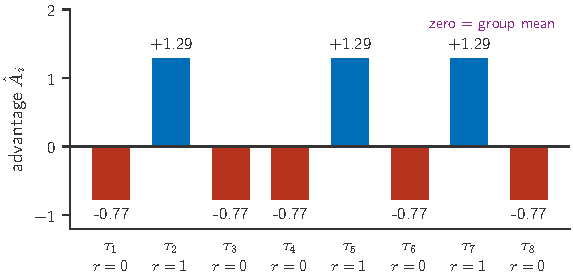
\includegraphics[width=0.82\textwidth]{s4-advantage.pdf}
  \vfill
  {\small \textcolor{valuecolor}{free value estimate}: no critic network (unlike PPO)}
\end{frame}

\begin{frame}{Push Up, Push Down}
  \vfill
  \centering
  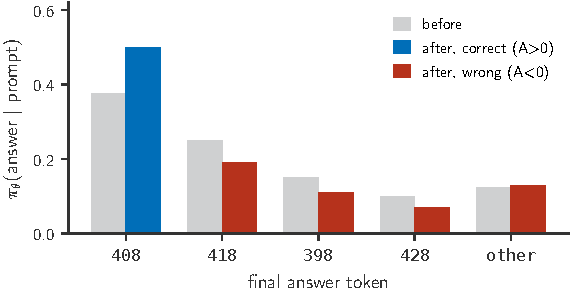
\includegraphics[width=0.82\textwidth]{s4-prob-shift.pdf}
  \vfill
  \begin{tabular}{@{}cc@{}}
    \textcolor{agentcolor}{$\hat A_i > 0$: raise $\log\pi_\theta$ of its tokens} &
    \textcolor{rewardcolor}{$\hat A_i < 0$: lower it}
  \end{tabular}
\end{frame}

\begin{frame}{GRPO in One Loop}
  \vfill
  \centering
  \begin{tikzpicture}[x=1cm, y=1cm, scale=1.05, transform shape, >={Stealth[length=3pt]}]
    % top row, left to right
    \node[rlbox=agentcolor, minimum width=2.4cm, minimum height=0.9cm] (pol) at (0, 1.1) {policy $\pi_\theta$};
    \node[rlbox=agentcolor, minimum width=2.6cm, minimum height=0.9cm] (smp) at (3.8, 1.1) {$G$ samples\\[-1pt]$\tau_1,\dots,\tau_G$};
    \node[rlbox=envcolor, minimum width=2.4cm, minimum height=0.9cm] (ver) at (7.6, 1.1) {verifier};
    % bottom row, right to left
    \node[rlbox=rewardcolor, minimum width=2.4cm, minimum height=0.9cm] (rew) at (7.6, -1.1) {rewards\\[-1pt]$r_1,\dots,r_G$};
    \node[rlbox=valuecolor, minimum width=2.6cm, minimum height=0.9cm] (adv) at (3.8, -1.1) {advantages\\[-1pt]$\hat A_1,\dots,\hat A_G$};
    \node[rlbox=agentcolor, minimum width=2.4cm, minimum height=0.9cm] (upd) at (0, -1.1) {update $\theta$};
    \draw[rlarrow] (pol) -- (smp);
    \draw[rlarrow] (smp) -- (ver);
    \draw[rlarrow] (ver) -- (rew);
    \draw[rlarrow] (rew) -- (adv);
    \draw[rlarrow] (adv) -- (upd);
    \draw[rlarrow] (upd) -- node[left, font=\scriptsize] {repeat} (pol);
    \node[font=\scriptsize, text=valuecolor!70!black] at (3.8, -2.15) {group mean as baseline};
  \end{tikzpicture}
  \vfill
\end{frame}

\begin{frame}{The GRPO Objective}
  \vfill
  \centering
  % vanilla form: no ratio, no clipping, no KL penalty
  {\large
  $\displaystyle
  \mathcal L(\theta) \;=\; -\,\frac1G\sum_{i=1}^{G}\textcolor{valuecolor}{\hat A_i}\;\textcolor{agentcolor}{\log\pi_\theta(\tau_i)}$}
  \\[12pt]
  {\normalsize
  $\displaystyle
  \textcolor{agentcolor}{\log\pi_\theta(\tau_i)} = \sum_{t}\log\pi_\theta(a_{i,t}\mid s_{i,t})
  \qquad
  \textcolor{valuecolor}{\hat A_i} = \frac{r_i-\operatorname{mean}(r_1,\dots,r_G)}{\operatorname{std}(r_1,\dots,r_G)}$}
  \vfill
  \begin{tikzpicture}[x=1cm, y=1cm]
    \node[s4vis=<2->, rlbox=valuecolor, text width=3.0cm, minimum height=1.1cm] at (0, 0) {\textbf{advantage}\\ better than its group?};
    \node[s4vis=<3->, rlbox=agentcolor, text width=3.0cm, minimum height=1.1cm] at (3.5, 0) {\textbf{log-prob of $\tau_i$}\\ every token it chose};
    \node[s4vis=<4->, rlbox=black, text width=3.0cm, minimum height=1.1cm] at (7.0, 0) {\textbf{minimize $\mathcal L$}\\ good $\tau$ up, bad $\tau$ down};
  \end{tikzpicture}
  \source{Simplified from Shao et al., 2024 (DeepSeekMath): ratio, clipping and KL penalty omitted}
  \vfill
\end{frame}

\begin{frame}{It Works}
  \vfill
  \centering
  {\large \textbf{DeepSeek-R1-Zero}}\\[2pt]
  {\small GRPO + verifiable rewards, no SFT data}
  \vfill
  {\normalsize AIME 2024 pass@1}
  \\[8pt]
  \begin{tikzpicture}[>={Stealth[length=5pt]}, scale=1.15, transform shape]
    \node[rlbox=humancolor, minimum width=3.4cm, minimum height=1.9cm, font=\fontsize{30}{34}\selectfont\bfseries, text=black] (a) at (0, 0) {15.6\%};
    \node[rlbox=agentcolor, minimum width=3.4cm, minimum height=1.9cm, font=\fontsize{30}{34}\selectfont\bfseries, text=agentcolor] (b) at (5.4, 0) {71.0\%};
    \draw[rlarrow=agentcolor, line width=2pt] (a) -- node[above, font=\small, text=black] {RL training} (b);
  \end{tikzpicture}
  \source{Guo et al., 2025 (DeepSeek-R1)}
  \vfill
\end{frame}
